\section{Prototype}
\label{section:prototyping}

Om te controleren of de detectiemethode die geselecteerd is in hoofdstuk~\ref{section:detection}
gebruikt kan worden om mogelijk op een tremor te reageren,
zal er een prototype gemaakt worden.
Dit hoofdstuk bevat een beschrijving van de keuzes die zijn gemaakt tijdens het maken van dit prototype;
hiermee beantwoordt het deels de vraag: Hoe kan de data die uit een detectie komt worden gebruikt?

\subsection{Wat wordt er gemaakt?}

De gekozen detectiemethode uit hoofdstuk~\ref{section:detection} is de EMG.
Om de bruikbaarheid van deze methode te testen, zal er een prototype worden gemaakt.
Gezien het doel van het onderzoek is om te mogelijkheid te verifiëren, ligt de focus niet op perfectie.
De richting zal vooral in theorie zijn, met mogelijke vervolgstappen in hoofdstuk~\ref{section:application}.

\subsection{Wat zijn bestaande oplossingen?}

Een EMG kan op verschillende manieren worden gedaan. 
Er wordt onderscheid gemaakt tussen drie soorten implementaties en twee systemen \cite{gohel2020}.

Desktop EMG-machines worden vooral gebruikt in een kliniek, ze zijn groot en accuraat;
deze zijn in kleiner draagbaar formaat te verkrijgen als Portable EMG's \cite{neurostyle2021,cadwell2023}.
In Figuur~\ref{figure:emgmachine} zijn deze EMG-vormen van CADWELL te zien \cite{cadwell2023}.

\begin{center}
    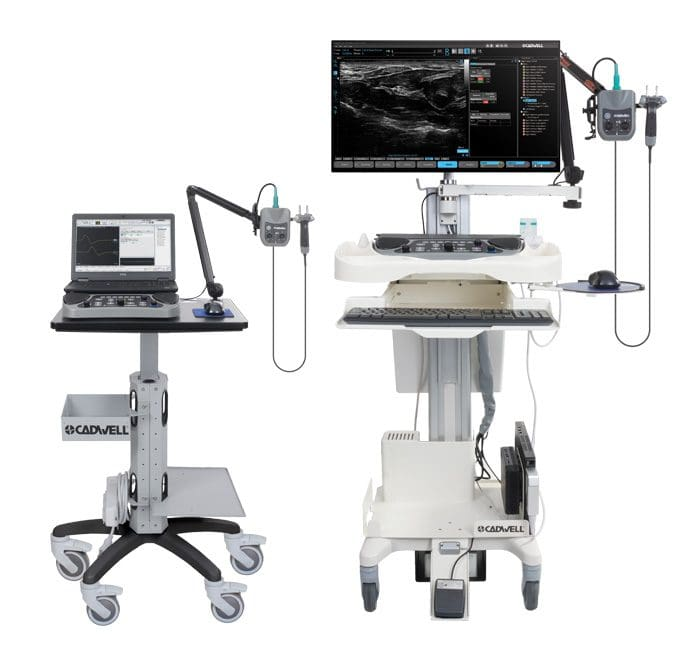
\includegraphics[width=0.4\textwidth]{./graphics/img-emgcarts.jpg}
    \captionof{figure}{Portable en Desktop EMG}
    \label{figure:emgmachine}
\end{center}

Een horloge variant van een EMG machine is verkrijgbaar om langdurig, of bij specifieke activiteiten, 
spieractiviteit te kunnen registreren en analyseren \cite{sips2024,activinsights2022}. 
Figuur~\ref{figure:emgwatch} toont de GENEActiv: Raw Data Accelerometer \cite{activinsights2022}.

\begin{center}
    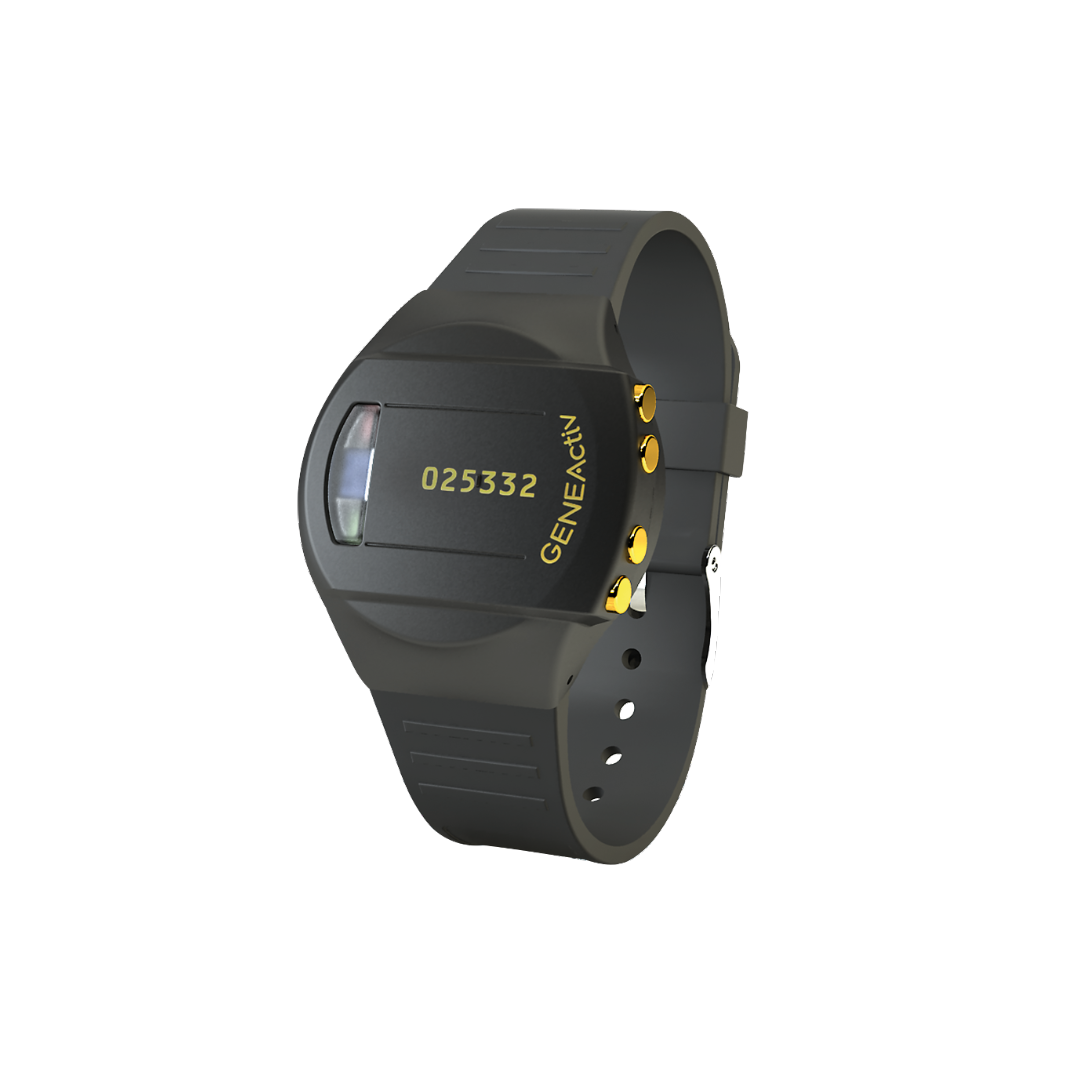
\includegraphics[width=0.4\textwidth]{./graphics/img-emgwatch.png}
    \captionof{figure}{GENEActiv: Raw Data Accelerometer}
    \label{figure:emgwatch}
\end{center}

Onder de system vallen draadloze systemen en geïntegreerde systemen \cite{gohel2020}.
De systemen vallen buiten de scope van dit onderzoek.

\subsection{Wat is er gebruikt?}

\subsection{Hoe is het gemaakt?}

\subsection{Wat kan het?}